\documentclass[../Homework]{subfiles}

\begin{document}
	\section{Estimating a Population Mean}
		\paragraph{1. Critical values}
			\begin{enumerate}[a.]
				\item
					\begin{align*}
						\df &= n - 1 = 9 \\
						t^* &= \left|\invT{\tarea{0.95} = 0.025}{9}\right| \approx 2.262
					\end{align*}
				\item
					\begin{align*}
						\df &= 20 - 1 = 19 \\
						t^* &= \left|\invT{\tarea{0.99} = 0.005}{19}\right| \approx 2.861
					\end{align*}
				\item
					\begin{align*}
						\df &= 77 - 1 = 76 \\
						t^* &= \left|\invT{\tarea{0.9} = 0.05}{76}\right| \approx 1.665
					\end{align*}
			\end{enumerate}
		\paragraph{3. Weeds among the corn}
			28 is less than 30 and the data contains outliers, so the Central Limit theorem does not take effect. Normality can therefore not be assumed.
		\paragraph{5. Check them all}
			\begin{enumerate}[a.]
				\item
					The Randomness condition is not met, as the sample contains all individuals from the same class. \\
					The 10\% condition is met, as my school contains more than 32\% people, so the sample size of 32 is less than 10\% of the population. \\
					The Normality condition met, as the sample size of 32 is greater than 30, so the Central Limit theorem is applicable.
				\item
					The Randomness condition is met, as each individual is randomly selected. \\
					The 10\% condition is met, as the city is large, so there were likely over 1000 home sales in the previous 6 months, so the sample size of 100 is less than 10\% of the population size. Independence is therefore justified. \\
			\end{enumerate}
		\paragraph{7. Blood pressure}
			\[s_{\bar{x}} = \frac{s_x}{\sqrt{n}} = \frac{9.3}{\sqrt{27}} \approx 1.79\]
			The means of random samples of size 27, the mean seated systolic blood pressure is expected to vary by about 1.79 from the true mean. \\\\
		\paragraph{9. Bone loss by nursing mothers}
			\begin{enumerate}[a.]
				\item
					\[\mu = \text{mean \% change in BMC of breast-feeding mothers over 3 months of breast-feeding}\]
					As a single parameter is concerned, a 1-sample $t$ interval should be constructed. \\
					The Randomness condition is met by the fact that this was a random sample. \\
					The 10\% condition is met, as there are far more than 470 breast-feeding mothers, so the sample size of 47 is less than 10\% of the population size. \\
					The Normality condition is met by the Central Limit theorem, which is applicable due to the sample size being 47, which is greater than 30. \\
					\begin{align*}
						\df &= n - 1 = 47 - 1 = 46 \\
						t^* &= \left|\invT{\tarea{0.99} = 0.005}{46}\right| \approx 2.687 \\
						s_{\bar{x}} &= \frac{s_x}{\sqrt{n}} = \frac{2.506}{\sqrt{47}} \approx 0.366 \\
						ME &= t^*s_{\bar{x}} \approx 2.687 \times 0.366 \approx 0.982 \\
						\cint &= \bar{x} \pm \ME \approx -3.587 \pm 0.982 \approx (-4.569, -2.605)
					\end{align*}
					It can be said with 99\% confidence that the true mean value $\mu$ of the percent change in BMC over 3 months of breast-feeding is contained within the interval $(-4.569, -2.605)$. \\
				\item
					The 99\% confidence interval provides convincing evidence of breast-feeding mothers on average losing bone mineral, as every value contained within the interval was negative.
			\end{enumerate}
		\paragraph{11. America's favorite cookie}
			\begin{enumerate}[a.]
				\item
					\[\mu = \text{mean weight of an Oreo cookie in grams}\]
					There is a single numerical value being tested, so a 1-sample $t$ interval should be constructed. \\
					The Randomness condition is met, as the sample is stated to be random. \\
					The 10\% condition is met, as more than 360 Oreo cookies exist, so the sample size of 36 is less than the population size. \\
					The Normality condition is met, as the sample size of 36 is greater than 30, so the Central Limit theorem is applicable.
					\begin{align*}
						\df &= n - 1 = 36 - 1 = 35 \\
						t^* &= \left|\invT{\tarea{0.9} = 0.05}{35} \right| \approx 1.6896 \\
						s_{\bar{x}} &= \frac{s_x}{\sqrt{n}} = \frac{0.0817}{\sqrt{36}} \approx 0.0136 \\
						ME &= t^*s_{\bar{x}} \approx 1.6896 \times 0.0136 \approx 0.023 \\
						\cint &= \bar{x} \pm \ME \approx 11.3921 \pm 0.023 \approx (11.3691, 11.4151)
					\end{align*}
					It can be said with 99\% confidence that the true mean value $\mu$ of the weight of an Oreo cookie is contained within the interval $(1.3691, 11.4151)$.
				\item
					Over many random samples of size 36 taken from the same population of all Oreo cookies, the true mean will be contained within $90\%$ of the $90\%$ confidence interval constructed about each sample mean.
			\end{enumerate}
		\paragraph{13. Pepperoni pizza}
			\[\mu = \text{ mean number of pepperonis on a large pepperoni pizza from their favorite pizza restaurant}\]
			There is a single numerical value, so a 1-sample $t$ interval should be constructed. \\
			The Randomness condition is met, as each time is stated to be random. \\
			The 10\% condition is met, as the restaurant likely made over 100 pizzas over the week, so the sample size of 10 is less than 10\% of the population size.
			The Normality condition is met, as the data lacks strong skew or outliers.
			\begin{align*}
				\df &= n - 1 = 10 - 1 = 9 \\
				t^* &= \left|\invT{\tarea{0.95} = 0.025}{9}\right| \approx 2.262 \\
				\bar{x} &= \frac{\sum x_i}{n} = \frac{374}{10} = 37.4 \\
				s_x &= \sqrt{\frac{\sum (x_i - \bar{x})^2}{n - 1}} \approx 7.662 \\
				s_{\bar{x}} &= \frac{s_x}{\sqrt{n}} \approx \frac{7.662}{\sqrt{10}} \approx 2.423 \\
				\ME &= t^*s_{\bar{x}} \approx 2.262 \times 2.423 \approx 5.481 \\
				\cint &= \bar{x} \pm \ME \approx 37.4 \pm 1.733 \approx (32.919, 42.881)
			\end{align*}
			It can be said with 95\% confidence that the true mean number of pepperoni slices on a large pepperoni pizza from Melissa and Madeline's favorite pizza restaurant is contained within the interval $(32.919, 42.881)$.
			\paragraph{15. A plethora of pepperoni}
				\begin{enumerate}[a.]
					\item
						The sample size of 10 is less than 30, so the Central Limit theorem could not be used to justify Normality.
					\item
						The interval contains 40, so there is not convincing evidence of the average number of pepperonis being less than 40.
						\item
							The margin of error could be reduced either by increasing the sample size, reducing $s_x$ and $s_{\bar{x}}$, or decreasing the confidence level, reducing $t^*$. The former would be more expensive while the latter would make the interval less likely to contain the true mean number of pepperonis.
				\end{enumerate}				
			\paragraph{17. Estimating BMI}
				\begin{align*}
					z^* &= \left|\invNormal{\tarea{0.99} = 0.005}{0}{1}{LEFT}\right| \approx 2.576 \\
					\ME &\ge z^*\sigma{\bar{x}} = z^*\frac{\sigma}{\sqrt{n}} \\
					n &\ge \left(\frac{z^*\sigma}{\ME}\right)^2 \approx \left(\frac{2.576 \times 7.5}{1}\right) \approx 373.213 \\
					n &= \lceil 373.213 \rceil = 374
				\end{align*}
			\paragraph{19. Willows in Yellowstone}
				\begin{enumerate}[a.]
					\item
						\begin{align*}
							s_{\bar{x}} &= \frac{s_x}{\sqrt{n}} \\
							s_x &= s_{\bar{x}}\sqrt{n} = 19.03\sqrt{23} \approx 91.265
						\end{align*}
					\item
						\[C = \tCDF{-1}{1}{23 - 1 = 22} \approx 0.672\]
				\end{enumerate}
			\paragraph{21.}\ \\
			$z$ can only be used when the population standard deviation is already known, so the answer is \textbf{b}.
			\paragraph{22.}
				\begin{align*}
					\df &= n - 1 = 23 - 1 = 22 \\
					t^* &= \left|\invT{\tarea{0.98} = 0.01}{22}\right| \approx 2.508
				\end{align*}
				The answer is therefore \textbf{e}.
			\paragraph{23.}\ \\
				The margin of error is minimized when $s_{\bar{x}}$ and $t^*$ are minimized. These are in turn minimized when $n$ is maximized and $C$ is minimized so the answer is \textbf{b}.
			\paragraph{24.}\ \\
				The most significant detriment to the validity of a $t$ interval listed is the data containing a clear outlier, as that would mean that the data fails to satisfy the Normality condition. (The Central Limit theorem is not applicable, as the sample size of 24 is less than the 30 required for it to take effect.) The answer is therefore \textbf{a}.
		\section{Estimating a Difference in Means}
			\paragraph{31. Is red wine better than white wine}
				\begin{enumerate}[a.]
					\item
						Both distributions are slightly skewed left without any outliers. The center of the white distribution appear lower than that of the red, while its minimum and maximum are both lower than those of the red distribution. \\
					\item
						\begin{align*}
							\mu_R &= \text{mean percent change in polyphenol levels for healthy men that drink red wine} \\
							\mu_W &= \text{mean percent change in polyphenol levels for healthy men that drink white wine} \\
							\diff{\mu} &= \mu_{R - W}
						\end{align*}
						As there are two quantitative values, a two-sample $t$ interval should be constructed. \\
						The Randomness condition is met, as the assignment was random. \\
						The 10\% condition is met, as there are over 900 healthy men that drink red wine, and the same is true of white wine, which means that the sample size of 9 is less than 10\% of each population. \\
						The Normality condition is met, as both distributions have little skew and lack outliers.
						\begin{align*}
							s_{\bar{x}_W - \bar{x}_R} &= \meandiff{s_W}{n_W}{s_R}{n_R} \approx \meandiff{2.517}{9}{3.292}{9} \approx 1.381 \\
							\df &= \dfdiff{s_{\bar{x}_R - \bar{x}_W}}{s_R}{n_R}{s_W}{n_W} \approx \dfdiff{1.381}{2.517}{9}{3.292}{9} \approx 14.971 \\
							t^* &= \left|\invT{\tarea{0.9} = 0.05}{\approx 14.971}\right| \approx  1.753 \\
							\ME &= t^*s_{\bar{x}_W - \bar{x}_R} \approx 1.753 \times 1.381 \approx 2.422 \\
							\diff{\bar{x}} &= \bar{x}_W - \bar{x}_R \approx 5.5 - 0.233 = 5.267 \\
							\cint &= \diff{\bar{x}} \pm \ME \approx 5.267 \pm 2.422 \approx (2.845, 7.689)
						\end{align*}
						It can be said with 90\% confidence that the true mean difference between the percent change in polyphenol levels of healthy men drinking red and white wine $\mu_{R - W}$ is contained within the interval $(2.845, 7.689)$.
				\end{enumerate}
			\paragraph{33. Paying for college}
				\begin{enumerate}[a.]
					\item
						Earnings cannot be negative, yet the standard deviations of each group is almost as large as their means. Regardless, as the sample sizes of both groups is greater than 30, the Central Limit theorem applies, so Normality can be justified.
					\item
						\begin{align*}
							\mu_M &= \text{mean earnings of male university students with summer jobs in \$} \\
							\mu_W &= \text{mean earnings of females university students with summer jobs in \$} \\
							\diff{\mu} &= \mu_{M - W}
						\end{align*}
						The Randomness condition is met, as the sample was random and independent. \\
						The 10\% condition is met, as there are more than $6,750$ university students with summer jobs that are male/female, so the sample sizes of 675 and 621 are both less than 10\% of their respective populations. \\
						The Normality condition is met, as stated in part a. \\
						\begin{align*}
							s_{\bar{x}_M - \bar{x}_W} &= \meandiff{s_M}{n_M}{s_W}{n_W} = \meandiff{1368.37}{675}{1037.46}{621} \approx 67.136 \\
							\df &= \dfdiff{s_{M - W}}{s_M}{n_M}{s_W}{n_W} \approx \dfdiff{67.136}{1368.37}{675}{1037.46}{621} \approx 1249.213 \\
							t^* &= \left|\invT{\tarea{0.9} = 0.05}{\approx 1249.213}\right| \approx 1.646 \\
							\ME &= t^*s_{M - W} \approx 1.646 \times 67.136 \approx 110.51 \\
							\diff{\bar{x}} &= \bar{x}_M - \bar{x}_W = 1884.52 - 1360.39 \approx 524.13 \\
							\cint &= \diff{\bar{x}} \pm \ME \approx 523.13 \pm 110.51 \approx (413.62, 634.64)
						\end{align*}
						It can be said with 90\% confidence that the true mean dollar difference between the earnings of male and female university students with summer jobs $\mu_{M - W}$ is contained within the interval $(413.62, 634.64)$.
				\end{enumerate}
			\paragraph{35. Reaction times}
				\begin{enumerate}[a.]
					\item
						The confidence interval does not provide convincing evidence of a difference in the true mean reaction times of athletes and non-athletes, as its contains 0, meaning that there is a chance of the difference being 0.
					\item
						It does not provide convincing evidence of a difference not existing, as not only are nonzero values contained, but the interval is centered above zero.
					\item
						To decrease the width of a confidence interval, the margin of error must be decreased, so $n$ must be increased, reducing the standard error, or the confidence level must be decreased, reducing $t^*$. The former is makes data collection more time-consuming and/or expensive while the latter makes the true mean less likely to be contained within the interval.
				\end{enumerate}
			\paragraph{37. Groovy tires}
				\begin{enumerate}[a.]
					\item
						\
						\begin{center}
							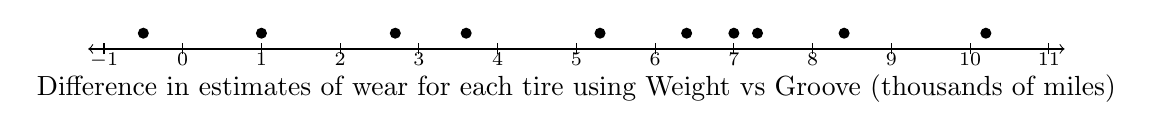
\begin{tikzpicture}
								\draw[<->] (-1.2, 0) -- (11.2, 0);
								\foreach \x in {-1,...,11} \draw (\x, -2pt) -- (\x, 2pt) node[below, font = \scriptsize]{$\pgfmathprintnumber {\x}$};
								\node at (5, -0.5){Difference in estimates of wear for each tire using Weight vs Groove (thousands of miles)};
								\fill (10.2, 0.2) circle (2pt);
								\fill (2.7, 0.2) circle (2pt);
								\fill (6.4, 0.2) circle (2pt);
								\fill (5.3, 0.2) circle (2pt);
								\fill (7, 0.2) circle (2pt);
								\fill (7.3, 0.2) circle (2pt);
								\fill (3.6, 0.2) circle (2pt);
								\fill (-0.5, 0.2) circle (2pt);
								\fill (8.4, 0.2) circle (2pt);
								\fill (1, 0.2) circle (2pt);
							\end{tikzpicture}
						\end{center}
					\item
						The distribution appears to be centered around 7 rather than 0, implying that the two methods give different estimates of tire wear on average.
					\item
						\begin{align*}
							\diff{\bar{x}} &\approx 4.556 & \diff{s} &\approx 3.226
						\end{align*}
						Using the weight method to estimate wear yields an estimate on average 4.556 thousand miles greater than that using the groove method.
				\end{enumerate}
			\paragraph{41. Groovy tires}
				\begin{align*}
					\mu_W &= \text{ mean estimate of wear using the weight technique (thousands of miles)} \\
					\mu_G &= \text{ mean estimate of wear using the groove technique (thousands of miles)} \\
					\diff{\mu} &= \mu_{W - G}
				\end{align*}
				The values for the differences can be individually analyzed, so a 1-sample $t$ test can be used. \\
				The Randomness condition is met, as the samples are random. \\
				The 10\% condition is met, as each technique has been used over 160 times, so the sample sizes of 16 is less 10\% of each population size. \\
				The Normality condition is met, as the distribution of the difference is symmetrical without outliers.
				\begin{align*}
					\df &= n - 1 = 16 - 1 = 15 \\
					t^* &= \left|\invT{\tarea{0.95} = 0.025}{15}\right| \approx 2.131 \\
					s_{\bar{x}_W - \bar{x}_G} &= \frac{\diff{s}}{n} \approx \frac{3.226}{\sqrt{16}} \approx 0.807 \\
					\ME &= t^*s_{\bar{x}_W - \bar{x}_G} \approx 2.131 \times 0.807 \approx 1.719 \\
					\cint &= \diff{x} \pm \ME \approx 4.556 \pm 1.719 \approx (2.837, 6.275)
				\end{align*}
				It can be said with 95\% confidence that the true mean difference between the wears predicted by the weight and groove methods (in miles) contained within the interval $(2.837, 6.275)$.
			\paragraph{43. Does playing piano make you smarter?}
				\begin{enumerate}[a.]
					\item
						\begin{align*}
							\mu_B &= \text{mean reasoning score of preschool children before 6 months of piano lessons} \\
							\mu_A &= \text{mean reasoning score of preschool children after 6 months of piano lessons.} \\
							\diff{\mu} &= \mu_{A - B}
						\end{align*}
						As the difference is being dealt with as a single value rather than the difference of two means, a 1-sample $t$ test should be performed. \\
						The Randomness condition is met, as sample was taken randomly. \\
						The 10\% condition is met, as there are more than 340 preschoolers, so the sample size of 34 is less than 10\% of the population size. \\
						The Normality condition is met, as 34 is greater than 30, so the Central Limit theorem can be applied.
						\begin{align*}
							\df &= n - 1 = 34 - 1 = 33 \\
							t^* &= \left|\invT{\tarea{0.9} = 0.05}{33}\right| \approx 1.692 \\
							s_{\bar{x}_A - \bar{x}_B} &= \frac{\diff{s}}{\sqrt{n}} = \frac{3.055}{\sqrt{33}} \approx 0.532 \\
							\ME &= t^*s_{\bar{x}_A - \bar{x}_B} \approx 1.692 \times 0.532 \approx 0.9\\
							\cint &= \diff{\bar{x}} \pm \ME \approx 3.618 \pm 0.9 \approx (2.718, 4.518)
						\end{align*}
						It can be said with 90\% confidence that the true mean difference change in reasoning scores of preschool children after 6 months of piano lessons is contained within the interval $(2.718, 4.518)$.
					\item
						The 90\% confidence interval provides convincing evidence that 6 months of piano lessons may result in an increase in the average reasoning scores of preschoolers, as it only contains positive values.
				\end{enumerate}
			\paragraph{45. Chewing gum}
				\begin{enumerate}[a.]
					\item
						The reason that the is paired is that every individual had data collected for both treatments.
					\item
						The Randomness condition is met, as the volunteers were randomly assigned. \\
						The 10\% condition is met, as over far more than 300 people exist, so the sample sizes of 30 are far less than 10\% of the population size. \\
						The Normality condition is met, as a sample size of 30 is exactly large enough for the Central Limit theorem to take effect.
					\item
						It can be said with 95\% confidence that the true mean difference in the number of words remembered when using or not using gum is contained within the interval $(-0.67, 1.54)$.
					\item
						The interval does not provide convincing evidence of chewing gum helping with short-term memory, as it contains 0, implying that there may be no difference.
				\end{enumerate}
			\paragraph{49.}\ \\
				A 1-sample $t$ interval is better for paired data, so the answer is \textbf{d}.
			\paragraph{50.}
				\begin{align*}
					\df &= n - 1 = 10 - 1 = 9 \\
					t^* &= \left|\invT{\tarea{0.95} = 0.0025}{9}\right| \approx 2.262 \\
					s_{\bar{x}_A - \bar{x}_B} &= \frac{s_{A - B}}{\sqrt{n}} = \frac{0.83}{\sqrt{10}} \\
					\ME &= t^*s_{\bar{x}_A - \bar{x}_B} \approx 2.262\left(\frac{0.83}{\sqrt{10}}\right) \\
					\cint &= \diff{\bar{x}} \pm \ME
				\end{align*}
				The answer is therefore \textbf{e}.
			\paragraph{51.}\ \\
			0 being contained within the interval means that there is a chance that the true difference is 0 and there being no difference, so the answer is \textbf{b}.
			\paragraph{52.}
				\begin{align*}
					s_{\bar{x}_A - \bar{x}_J} &= \meandiff{s_A}{n_A}{s_J}{n_J} \approx \meandiff{2.4}{30}{2.26}{30} \approx 0.602 \\
					\df &= \dfdiff{s_{\bar{x}_A - \bar{x}_J}}{s_A}{n_A}{s_J}{n_J} \approx \dfdiff{0.602}{2.4}{30}{2.26}{30} \approx 57.792 \\
					t^* &= \left|\invT{\tarea{0.95} = 0.025}{\approx 57.792}\right| \approx 2.002 \\
					\ME &= t^*s_{\bar{x}_A - \bar{x}_J} \approx 2.002\meandiff{2.4}{30}{2.26}{30} \\
					\cint &= \diff{\bar{x}} \pm \ME
				\end{align*}
				The answer is closest to \textbf{d}.
\end{document}